\chapter{Conclusions}

\section{Summary of the project and project Plan}
Currently, the project is still at the stage of designing modeling attack, which is the first part of objectives mentioned in Chapter 1. As stated in Chapter 4, 
reinforcement learning and GAT still suffer from implementation problems. The overall project plan is display in Figure \ref{fig:figure13}.
\begin{figure}[htp]
    \centering
    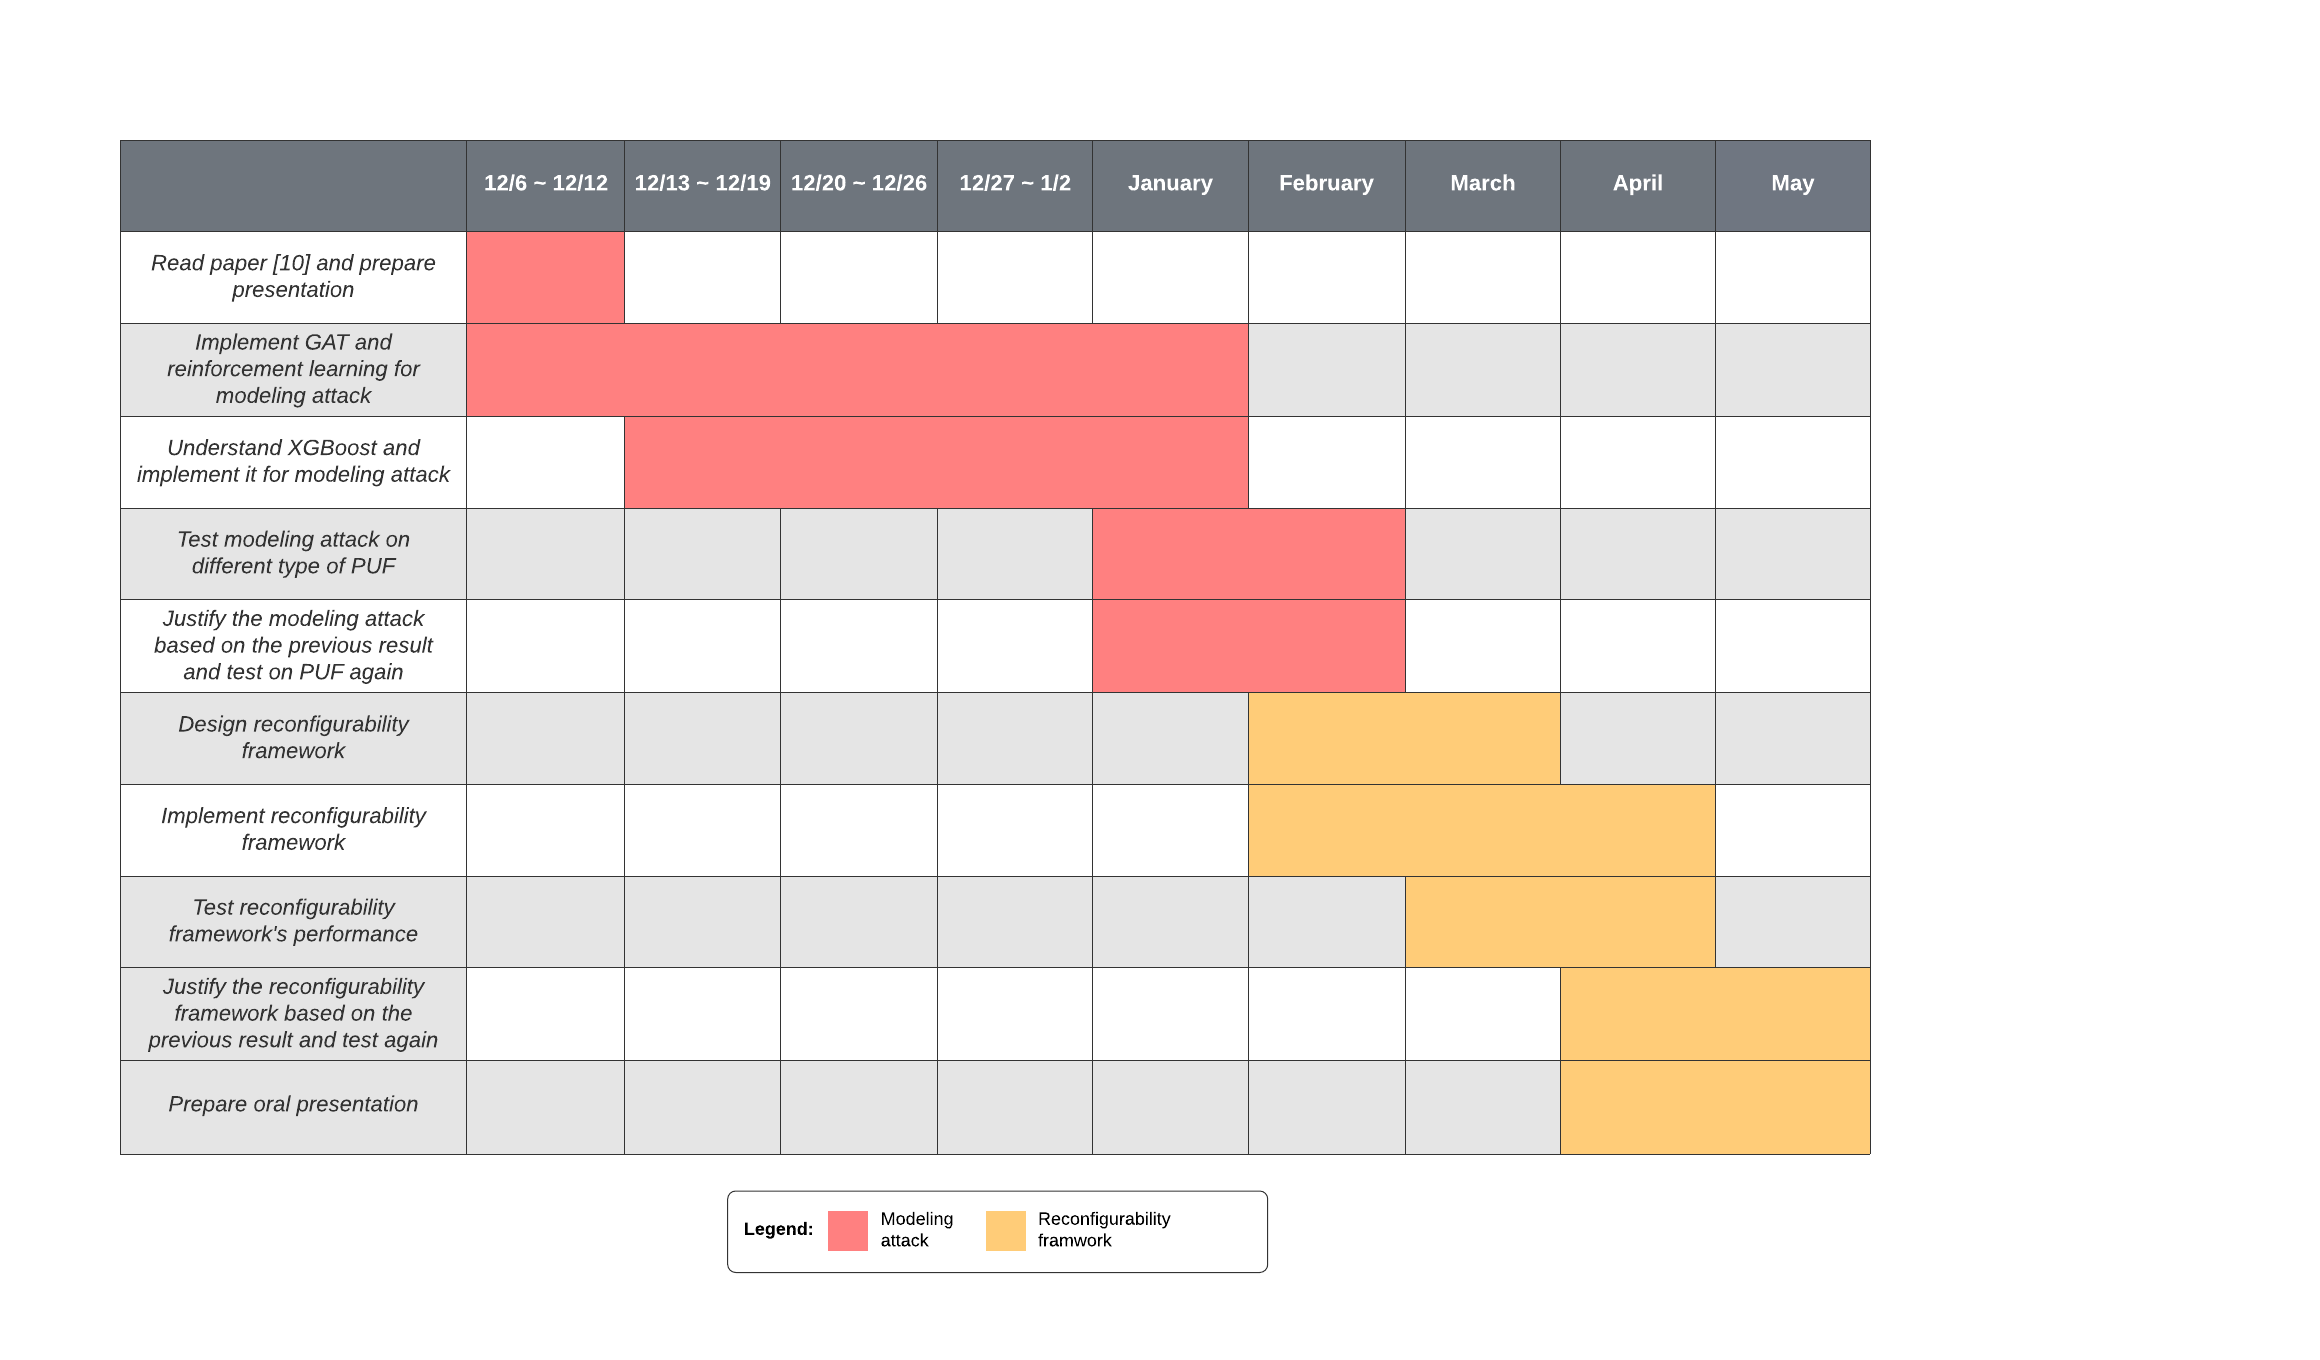
\includegraphics[width=22cm]{figures/project_plan.png}
    \caption{Gantt chart for project's plan}
    \label{fig:figure13}
    \end{figure}

\subsection{Short term plan}
For the short term goal, in the next few weeks till 12/22's meeting,
the main task is to successfully implement modeling attack mentioned in Chapter 4 or other methods that can achieve prediction accuracy higher than 80\%. The XGBoost was a new idea to try if both the previous machine learning fail to implement or model the arbiter PUF. 
However, more research on XGBoost was required. In addition, investigate more about pypuf, and try fully understand the paper \cite{Reference11}, then prepare a presentation for 12/22's meeting.

\subsection{Long term plan}
In the long term, after the modeling attack is implemented, start on designing a reconfigurability framework to prevent the attack. The framework that was mentioned in Chapter 2 and Chapter 3 will be considered. The framework
is expected to be completely implemented at the end of March 2022 so there will have enough time for testing and writing dissertation.
